\section{Introduction}\label{sec-intro}
First of all, this hotel is a hypothetical organisation, like I just mentioned. It aims to train hoteliers, a hotel with creativity and the spirit of a TULIP lab. This hotel stores all and if the hotel website's web traffic and data about the various relevant web pages used by users.

\section{Data cleaning}\label{sec-intro}

	Extract the obtained data set: The obtained data set is in the form of a compressed package, which should be decompressed first.
	The names of the data sets in the log format of all the compressed packages shown in Figure 1 were obtained, and the statistics were carried out to find that there were 120 files in total.

\begin{table}  \centering
  \caption{DATA ATTRIBUTE}
  \label{tbl:overall-experiments}
  \begin{tabular}{ccc}
\toprule
    % after \\: \hline or \cline{col1-col2} \cline{col3-col4} ...
    Attribute Name &Description& Examples \\
\midrule
   date & Date of user access & 1/11/2006 \\
    time & User access specific time & 12:00:08 AM \\
    s-ip &provides information on various protocols to the transport layer. & 127.0.0.1 \\
    sc-status & Server successfully returns web page & 200\\

\bottomrule
\end{tabular}
\end{table}



	\begin{figure}
		\centering
		\selectcolormodel{rgb}
		%\missingfigure{Testing.}
		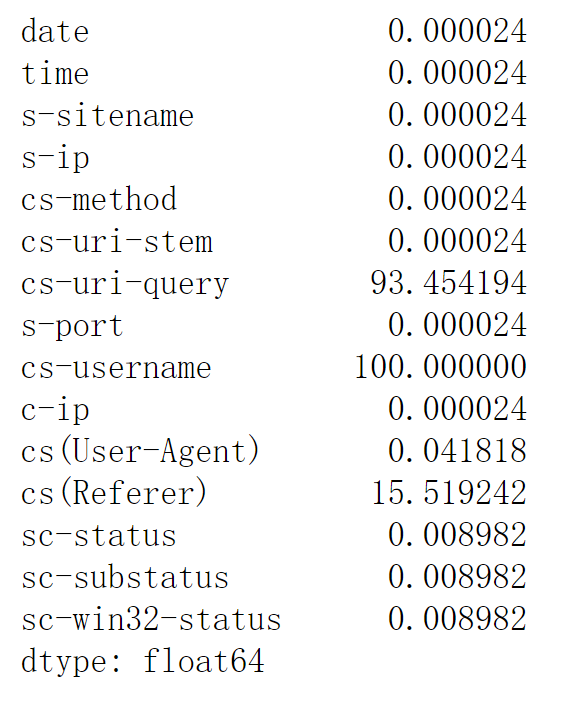
\includegraphics[width=0.6\textwidth]{Capture5.png}\\
		\caption{loading}\label{fig:loading}
	\end{figure}

\section{Data  visualization }\label{sec-intro}

\begin{figure}
	\centering
	\selectcolormodel{rgb}
	%\missingfigure{Testing.}
	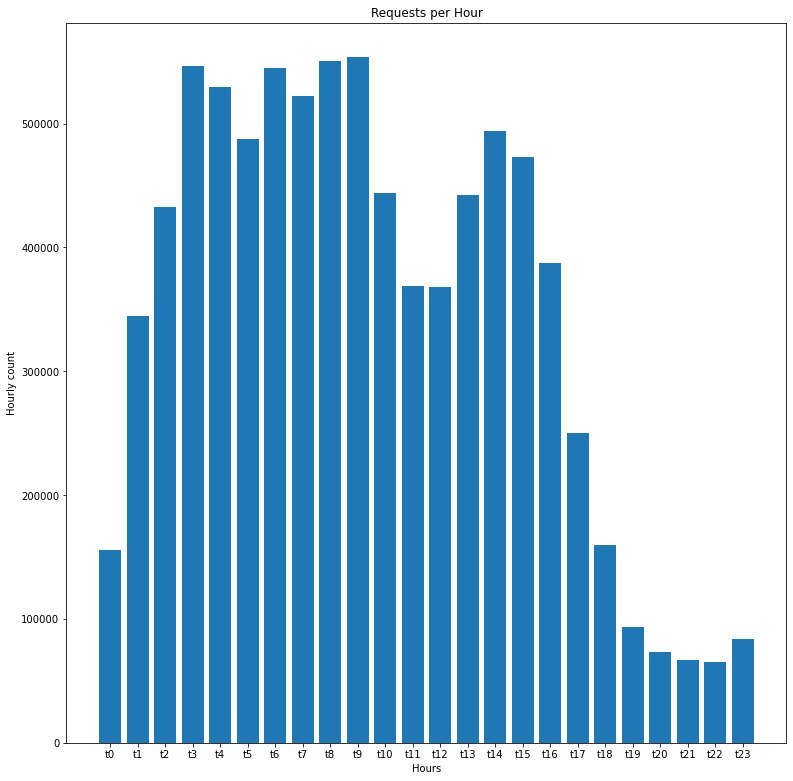
\includegraphics[width=0.6\textwidth]{ll1.png}\\
	\caption{loading}\label{fig:loading}
\end{figure}
First of all, I analyzed the click traffic.
This is mainly for each hour to carry out statistics.
Speaking each hour the same row counts as the flow plotted out.
We can get some very interesting information. Due to the time difference, Melbourne time is adopted here, and we can see that there are more than 400,000 visitors in Melbourne time, and then there is a small peak from 2 to 9 in the morning, and then from 1 to 3 in the afternoon.
There are also fewer visits between 7pm and 11pm

\begin{figure}
	\centering
	\selectcolormodel{rgb}
	%\missingfigure{Testing.}
	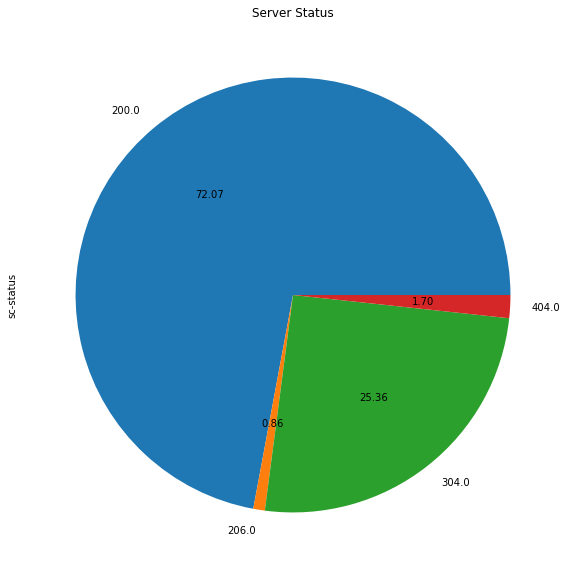
\includegraphics[width=0.4\textwidth]{ll2.png}\\
	\caption{loading}\label{fig:loading}
\end{figure}
In the second step, I made statistics on the protocol status of the page visited by the user.
Six million people were the most successful.
In second place is rendering 304, which means the server has a cache for the web page.
This proves that the user has visited the site for the second or more times.


\twocolumn{
\begin{figure}
	\centering
	\selectcolormodel{rgb}
	%\missingfigure{Testing.}
	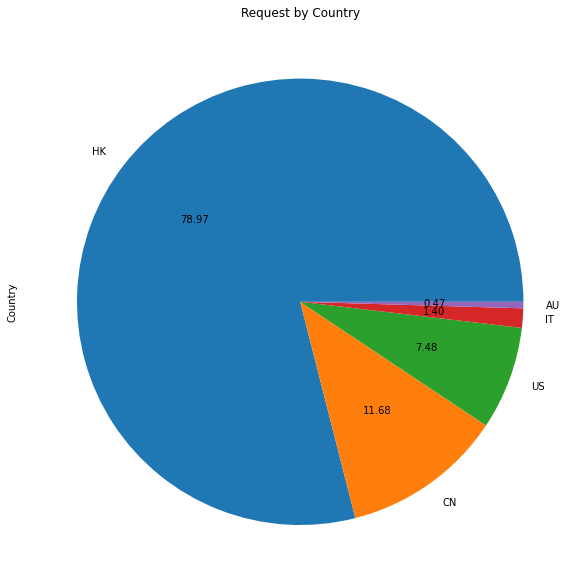
\includegraphics[width=0.6\textwidth]{ll3.png}\\
	\caption{loading}\label{fig:loading}
\end{figure}
The third step is to analyze the IP of users logging in the website, mainly from the perspective of country and city.
You want to know the likelihood of a potential user's location.
The first is the state.
I found that Hong Kong, China and the United States are the top three countries to visit.
Hong Kong is the majority, so re-marketing can focus on these three countries.
}{
\begin{figure}
	\centering
	\selectcolormodel{rgb}
	%\missingfigure{Testing.}
	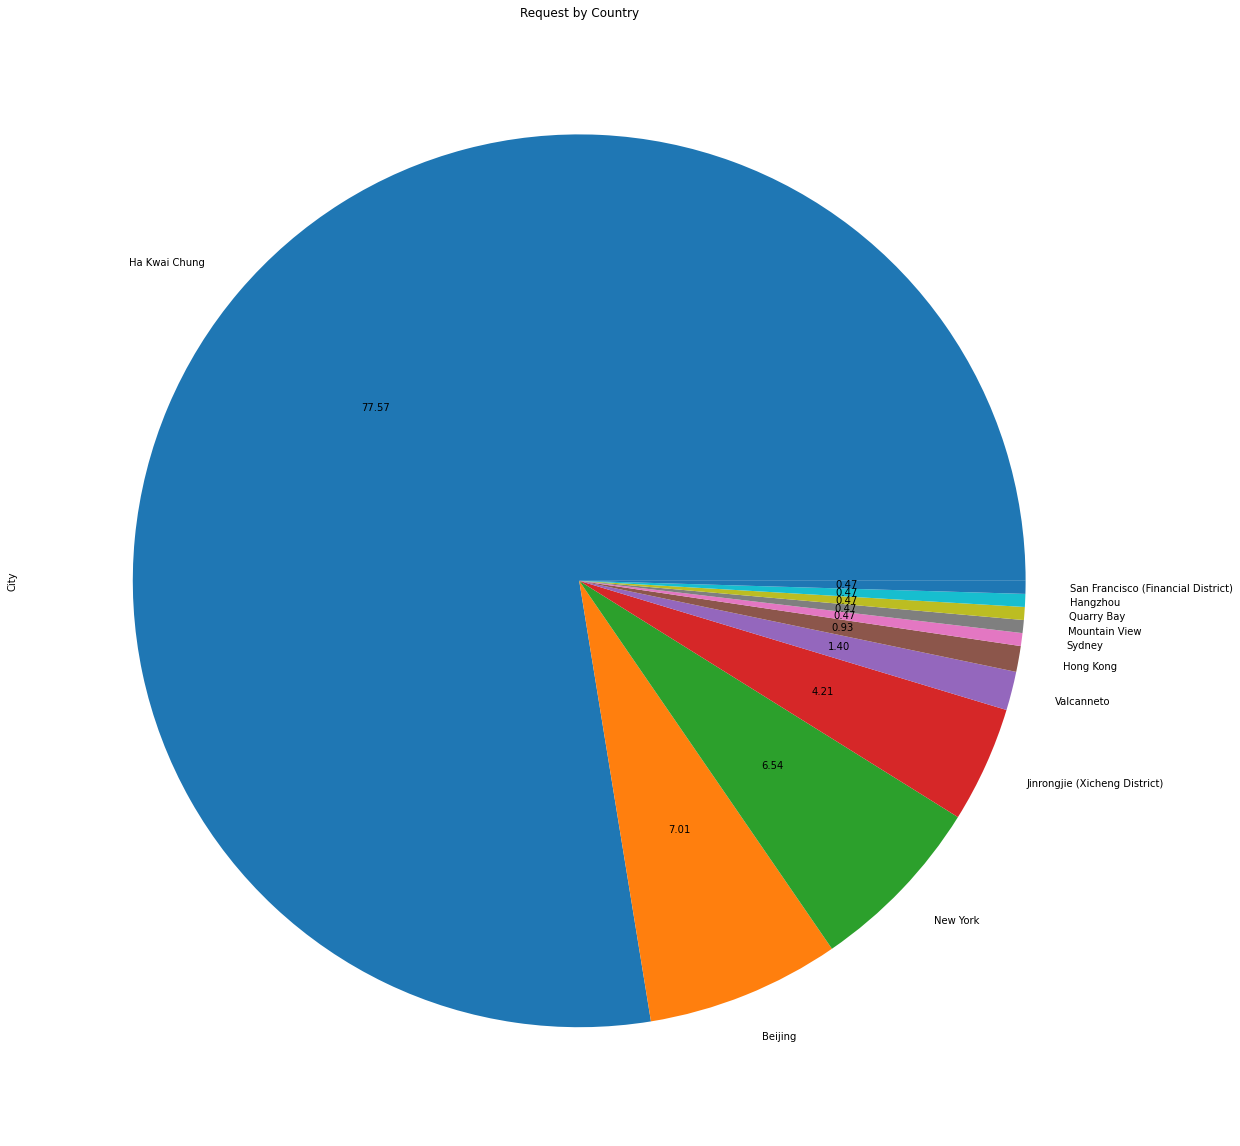
\includegraphics[width=0.6\textwidth]{ll4.png}\\
	\caption{loading}\label{fig:loading}
\end{figure}

when we look at the cities, we find that the first-tier cities of these three countries are the main visitors, such as Beijing in China and New York in the United States.
}



\section{Conclusions} \label{sec-conclusions}
So just to recap a little bit, the reason I did all four of these analyses was to try to understand how often people were visiting over that time period, how often they were visiting, whether they were first-time visitors or repeat visitors.
The main purpose of geographical analysis is to find out the geographical location of potential users, expand the market, and adjust the development strategy and planning of the organization in time.








